\documentclass[a4paper,10pt,twoside]{article}

\usepackage[top=1in, bottom=1in, left=1in, right=1in]{geometry}
\usepackage[utf8]{inputenc}
%\usepackage[spanish,es-ucroman,es-noquoting]{babel}
\usepackage{fancyhdr}
\usepackage{lastpage}
\usepackage{graphicx}



% Evita que el documento se estire verticalmente para ocupar
% el espacio vacío en cada página.
%\raggedbottom


%%%%%%%%%% Configuración de Fancyhdr - Inicio %%%%%%%%%%
\pagestyle{fancy}
\thispagestyle{fancy}
\lhead{TP2, Organización del Computador II}
\renewcommand{\footrulewidth}{0.4pt}
\cfoot{\thepage /\pageref{LastPage}}

\fancypagestyle{caratula} {
   \fancyhf{}
   \cfoot{\thepage /\pageref{LastPage}}
   \renewcommand{\headrulewidth}{0pt}
   \renewcommand{\footrulewidth}{0pt}
}
%%%%%%%%%% Configuración de Fancyhdr - Fin %%%%%%%%%%


\begin{document}


%%%%%%%%%%%%%%%%%%%%%%%%%%%%%%%%%%%%%%%%%%%%%%%%%%%%%%%%%%%%%%%%%%%%%%%%%%%%%%%
%% Carátula                                                                  %%
%%%%%%%%%%%%%%%%%%%%%%%%%%%%%%%%%%%%%%%%%%%%%%%%%%%%%%%%%%%%%%%%%%%%%%%%%%%%%%%


\thispagestyle{caratula}

\begin{center}


\includegraphics[height=2cm]{DC.png} 
\hfill

\includegraphics[height=2cm]{UBA.jpg} 

\vspace{2cm}

Departamento de Computación,\\
Facultad de Ciencias Exactas y Naturales,\\
Universidad de Buenos Aires

\vspace{4cm}

\begin{Huge}
Trabajo Pr\'actico Nro 3\\
\end{Huge}
\begin{Huge}
System Programming - TronTank
\end{Huge}

\vspace{0.5cm}

\begin{Large}
Organización del Computador II
\end{Large}

\vspace{1cm}

Primer Cuatrimestre de 2014

\vspace{4cm}

Grupo: \textbf{Colombia - Arepa}

\vspace{0.5cm}

\begin{tabular}{|c|c|c|}
\hline
Apellido y Nombre & LU & E-mail\\
\hline
Cisneros, Rodrigo 			& 920/10 & rodricis@hotmail.com\\
Rodr\'iguez, Agust\'in	& 120/10 & agustinrodriguez90@hotmail.com\\
Tripodi, Guido		& 843/10 & guido.tripodi@hotmail.com\\
\hline
\end{tabular}

\end{center}

\newpage


%%%%%%%%%%%%%%%%%%%%%%%%%%%%%%%%%%%%%%%%%%%%%%%%%%%%%%%%%%%%%%%%%%%%%%%%%%%%%%%
%% Índice                                                                    %%
%%%%%%%%%%%%%%%%%%%%%%%%%%%%%%%%%%%%%%%%%%%%%%%%%%%%%%%%%%%%%%%%%%%%%%%%%%%%%%%


\tableofcontents

\newpage


%%%%%%%%%%%%%%%%%%%%%%%%%%%%%%%%%%%%%%%%%%%%%%%%%%%%%%%%%%%%%%%%%%%%%%%%%%%%%%%
%% Introducción                                                              %%
%%%%%%%%%%%%%%%%%%%%%%%%%%%%%%%%%%%%%%%%%%%%%%%%%%%%%%%%%%%%%%%%%%%%%%%%%%%%%%%


\section{Introducción}
En el siguiente informe se describen los m\'odulos implementados que constituyen el c\'odigo del Trabajo Pr\'actico Nro 3 
\emph{TronTank}. Cada m\'odulo descripto incluye una breve descripci\'on de las decisiones de diseño tom\'adas por el grupo con 
respecto al procesador \emph{Intel} y sus reglas de desarrollo y, de ser necesario, una explicacion de la implementaci\'on. Esto incluye
en el TP: configuraci\'on de la GDT, pasaje a modo protegido, configuraci\'on de la IDT, paginaci\'on, TSS y la organizaci\'on del 
scheduler. 




%%%%%%%%%%%%%%%%%%%%%%%%%%%%%%%%%%%%%%%%%%%%%%%%%%%%%%%%%%%%%%%%%%%%%%%%%%%%%%%
%% Desarrollo                                                                %%
%%%%%%%%%%%%%%%%%%%%%%%%%%%%%%%%%%%%%%%%%%%%%%%%%%%%%%%%%%%%%%%%%%%%%%%%%%%%%%%

\newpage
\section{Desarrollo y Resultados}

\subsection{Ejercicio 1. GDT}

\subsubsection{Global Descriptor Table}
Como ya sabemos, el procesador inicia en ''modo real'', el cual direcciona a 1 MB de memoria y no posee niveles de protecci\'on ni privilegios.\\
Por eso necesitamos que el procesador pase a ''modo protegido'', para direccionar a m\'as memoria y poder manejar distintos niveles de protecci\'on. Nuestro kernel se encargar\'a de hacer esto.\\
\\
Antes de iniciar en modo protegido, es imprescindible tener bien configurado la Tabla de Descriptores Globales, la cual contiene a los descriptores de segmento, con el fin de definir caracter\'isticas de varias \'areas de la memoria.\\
En el enunciado se piden una segmentacion flat, con 4 segmentos que deben direccionar a 1.75 GB: 2 para c\'odigo de nivel 0 y 3 respectivamente, y 2 para datos, de nivel 0 y 3 tambi\'en.\\

La estructura de un descriptor de segmento es la siguiente:\\
\begin{itemize}
  \item L — 64-bit code segment (IA-32e mode only)
  \item AVL — Available for use by system software
  \item BASE — Segment base address
  \item D/B — Default operation size (0 = 16-bit segment; 1 = 32-bit segment)
  \item DPL — Descriptor privilege level
  \item G — Granularity
  \item LIMIT — Segment Limit
  \item P — Segment present
  \item S — Descriptor type (0 = system; 1 = code or data)
  \item TYPE — Segment type
\end{itemize}

Para definir los segmentos que nos requieren, los items importantes son:\\
\begin{itemize}
 \item BASE: este parametro indica el comienzo del segmento. En los 4 casos, este fue 0 ya que se pidió una segmentacion flat.
 \item P: Present, este parametro indica si el segmento est\'a presente en la memoria. El valor en los 4 segmentos es 0x01 ya que efectivamente estaban presentes.
 \item DPL: Nivel de privilegios del descriptor. Dado que se piden dos segmentos de código y dos de datos nivel 0 y nivel3, este 
parametro var\'ia seg\'un cual de estos queremos implementar. Nivel 0 implica DPL = 00b y nivel 3 implica DPL = 11b.
 \item G. Granularity. Este flag indica si el tamaño del descriptor es mayor o menor que 1 Mb. Esto sucede dado que solo se poseen 20 bits para 
indicar el tamaño del segmento. En particular, si G = 1 entonces el valor de los 20 bits ser\'a multiplicado por 4 Kb provocando que con 
 solo 20 bits pueda representar 4Gb de memoria. En nuestro caso queremos un tamaño de 1.75Gb entonces necesitamos G = 1.
 \item Limit: Tamaño del segmento. Va para los 4 segmentos lo mismo.\\
  \indent Tenemos que direccionar a 1.75 GB, que son 1792 MB, que equivalen a 1835008 KB.\\
  \indent Como G vale 0x01, las unidades deben representarse de 4 KB, por eso dividimos por 4.\\
  \indent $\frac{1835008}{4} = 458752$\\
  \indent Pero como la memoria empieza desde el 0, debe ser un n\'umero menos: 458751\\
  \indent $458751 = 0x6FFFF$
 \item Type: Indica si es un segmento de c\'odigo o de datos. Para el segmento de c\'odigo de nivel 0 ponemos el valor de 0x08, indicando 
que es ''Execute only''. para el segmento de c\'odigo de nivel 3 se usa 0x0A, \emph{Read / Execute}. Mientras que para los 2 de datos 
ponemos el valor de 0x02, indicando que son de Read/Write.
\end{itemize}

Tambi\'en se define un segmento que reservado para el \'area de la pantalla en la memoria. Sabemos que empieza en la direcci\'on base
0x000B8000, con un tamaño de 0x0F9F. Dado que se utilizar\'a como un segmemto de datos, su tipo es de Lectura/ Escritura.\\\\
\\
Tambi\'en necesitamos entradas para cada una de las tareas y sus banderas. Es decir, selectores de 
TSS. Estos ser\'an definidos de forma din\'amica y no hardcodeados, bas\'andose en la posici\'on de su respectivo TSS. B\'asicamente cada
una de estas entradas de la GDT para las TSS fue inicada de la siguiente manera:
\begin{itemize}
 \item BASE: Direcci\'on donde fue definido el comienzo de la TSS para cada respectiva tarea.
 \item P: Present. Este flag debe ir seteado para todas las TSS.
 \item DPL: las tareas corren en nivel 3, por lo tanto, el DPL = 3 salvo para las tareas INICIAL e IDLE que deben correr en nivel 0.
 \item limit: Como m\'inimo las TSS tienen un tamaño de 104 bytes es decir 0x67. Esto es como m\'inimo ya que existe la posibilidad de
extender el IO Map Base Address.
 \item type: este es particular. dado que es un tipo de descriptor de segmento, el valor tiene que ser 0x09.
 \item S: este flag determina si el descriptor se refiere a un segmento de c\'odigo o datos o si es de sistema. En este caso como los
descriptores de TSS son de sistema S = 0.
\end{itemize}



\subsubsection{Pasaje a modo protegido}

En funci\'on de pasar a ejecutar en modo protegido el manual de \emph{Intel}\footnote{Ver Intel 64 and IA-32 Architectures Software 
Developer's Manual, Volume 3 System Programming Guide} explicita una serie de pasos que se deben seguir para complir con esto.\\
\begin{itemize}
 \item Habilitar A20. al realizar esto habilitamos el acceso a direcciones superiores a 1 Mb de memoria.
 \item Una vez que tenemos configurada la gdt, guardamos su ubicacion en una variable gdt\_desc. Para que luego la instrucci\'on lgdt 
pueda cargar la direccion de comienzo de la GDT.
 \item Seteamos el flag PE del registro CR0, que indica ''Protected Envirnoment''.
 \item Por \'ultimo para pasar a modo protegido hacemos un jmp al comienzo del segmento de c\'odigo de nivel 0.
 \item Una vez ah\'i acomodamos todos los segmentos apuntando a datos de nivel 0 y seteamos la pila del Kernel en 0x27000 seg\'un lo
indicado por el enunciado.
\end{itemize}

\newpage
\subsection{Ejercicio 2 IDT}

\subsubsection{Interrupt Descriptor Table}
A trav\'es de la IDT, definimos donde est\'a el c\'odigo de las interrupciones que manejaremos.\\
La estructura de una entrada en la IDT est\'a definida en idt.h y en idt.c son iniciadas todas las entradas.\\
Por medio de una macro se cargan las primeras 19 interrupciones del procesador, que van desde la divisi\'on por 0 hasta la interrupci\'on SIMD.\\
Luego son completadas todas las entradas restantes de la tabla con entradas de interrupciones inv\'alidas con el prop\'osito de manejar 
de alguna forma todas las interrupciones posibles. Algunas de estas son definidas nuevamente:\\
\begin{itemize}
 \item Interrupci\'on 0x32: Clock.
 \item Interrupci\'on 0x33: Teclado.
 \item Interrupci\'on 0x52: Servicios del sistema (syscalls).
\end{itemize}

En isr.asm se encuentra el c\'odigo donde atendemos estas interrupciones. Saliendo de las 3 interrupciones mencionadas arriba (clock, teclado, syscall),
todas las interrupciones serán atendidas de una forma similar (para esto usamos un macro). Se realizan las escrituras pertinentes en pantalla y despues se desalojara la 
tarea que la causo.

La estructura de una entrada de la idt, definida en idt.h, es la siguiente:\\
\begin{itemize}
 \item offset\_0\_15: primeros 16 bits del offset al entry point, que atender\'a la interrupci\'on
 \item segsel: selector de segmento de codigo de nivel 0 la gdt
 \item attr: atributos de la entrada: Present, DPL, D. Esto var\'ian seg\'un si la interrupci\'on es de Reloj o Teclado que llevan DPL = 00b
o Servicios cuyo DPL = 11b.
 \item offset\_16\_31: segundos 16 bits del offset al entry point.
\end{itemize}


\begin{tabular}{l l l l l}
Indice & Descripcion & P & DPL & D\\

\hline
0...19 & Ins del procesador & 1 & 0 & 1 \\
32 & Clock & 1 & 0 & 1\\
33 & Teclado	 & 1 & 0 & 1\\
52 & Syscall & 1 & 3 & 1\\
\end{tabular}

\subsubsection{Proceso para activar interrupciones}

Para poder activar todas estas interrupciones y sus respectivos handlers se siguen los siguientes pasos:\\
\begin{itemize}
 \item Mediante el uso de la instrucci\'on LIDT [IDT\_DESC], cargamos el principio del array donde tenemos cargados todas las interrupciones
 \item Por \'ultimo se deshabilita, se resetea y se vuelve a habilitar el pic que obtiene las interrupciones.\footnote{Las funciones de 
deshabilitar, habilitar y resetear fueron provistas por la c\'atedra.}
\end{itemize}

\newpage
\subsection{Ejercicio 3. Paginaci\'on}

\subsubsection{Kernel, Identity Mapping}
Debemos mapear con Identity mapping las direcciones 0x00000000 a 0x00DC3FFF. Para esto fueron necesarios:

\begin{itemize}
 \item 1 Tabla de Directorios de p\'aginas que empieza en la direccion 0x27000.
 \item 4 Entradas de tabla de directorios. 
 \item 4 tablas de p\'aginas. La 3 primeras Page table posee sus 1024 entradas completas  
y tienen como base la direcci\'on 0x28000, 0x29000 y 0x2A000 respectivamente. Y la cuarta tabla con 452 entradas presentes desde la dirección 0x2B000. \\
De esta forma conseguimos mapear todas las direcciones
\end{itemize}

Las entradas de directorio para Kernel son cargadas de la siguiente manera\footnote{Se pueden considerar a los flags no declarados como
no seteados, es decir, iguales a 0.}:
\begin{itemize}
 \item P = 1.
 \item R/W = 1.
 \item U/S = 0.
 \item Direccion de la Page Table = 0x28000, 0x29000, 0x2A000 o 0x 2B000 seg\'un corresponda la  page table.
\end{itemize}

Las entradas de Page Table para el Kernel son cargadas de la siguiente manera\footnotemark[3]:
\begin{itemize}
 \item P = 1.
 \item R/W = 1.
 \item U/S = 0.
 \item Direccion del Page Frame desde 0x00000000 a 0x00DC3FFF seg\'un corresponda.
\end{itemize}

A continuaci\'on se detalla un esquema para una mejor comprensi\'on de lo explicado:

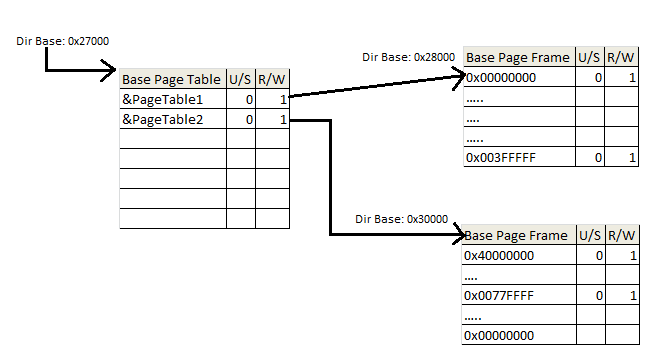
\includegraphics[scale=0.6]{imagenes/tablasDePaginasEj3.png}

\subsubsection{Activaci\'on de paginaci\'on}

Luego de armar el directorio de p\'aginas podemos habilitar la paginaci\'on. Para esto seguimo los siguientes pasos:
\begin{itemize}
 \item Cargar en CR3 la direccion al inicio del directorio de p\'aginas.
 \item Setear el bit mas significativo del registro CR0.
\end{itemize}


\newpage
\subsection{Ejercicio 4. Paginaci\'on de tareas}

\subsubsection{Paginaci\'on de las tareas}

Para la paginaci\'on de tareas se necesitaron los siguientes m\'odulos por cada tarea:
\begin{itemize}
 \item Inicializar un directorio de p\'aginas con 5 entradas, 4 para el Kernel iguales a las descriptas en el ejercicio 3 (es decir, identity mapping) 
 y otra entrada con dos entradas de tablas presentes para direccionar a las p\'aginas de c\'odigo y pilas de cada tarea. Este Page directory est\'a definido en la direccion 0x00100000
 \item Dentro de la Page Table de las tareas se encuentran definidas las entradas de cada p\'agina de la tarea. 
\end{itemize}

Con el fin de simplificar la cantidad de pasos, las direcciones fisicas de las paginas cada tarea estaran mapeadas en arrays externos. De esta forma no
tendremos que buscar dentro de la GDT para buscar una direccion fisica a la hora de hacer otras operaciones, que puede ser costoso en cuestiones de tiempo
y dejar un codigo poco claro.

A diferencia del ejercicio anterior, como en este caso estamos mapeando tareas, estas se diferencian de las p\'aginas de Kernel en que
los attributos que utilizan son diferentes, es decir, las tareas al correr en nivel 3 requieren que sus Page Directory entries y sus
Page table entries posean U/S = 1. De lo contrario no puedo acceder a esas p\'aginas como nos lo demostro\'o nustra experiencia en la
implementaci\'on.

El siguiente esquema explica mas simplemente lo nombrado anteriormente. Tener en cuenta que esto debe realizarse por cada tarea y que si
bien cada una est\'a mapeada al mismo lugar, la base del Page Directory es distinto para cada tarea, provocando que cada una tenga su
propio mapeo. %Para empezar, page directory entry que corresponde a la tarea, es la 0x100 ya que 0x40000000 es una direccion virtual entonces
%la tenemos que decodificar como 

\begin{center}
  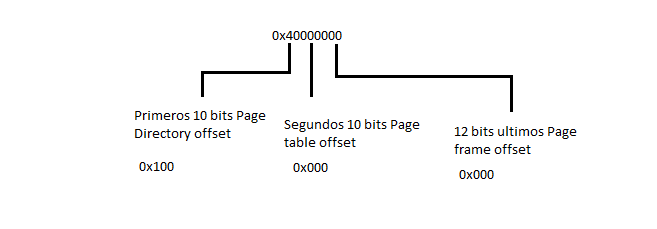
\includegraphics[scale=0.6]{imagenes/ComoDividoVirtual.png} 
\end{center}

Y Luego de esto el esquema de paginaci\'on nos quedar\'ia algo as\'i:

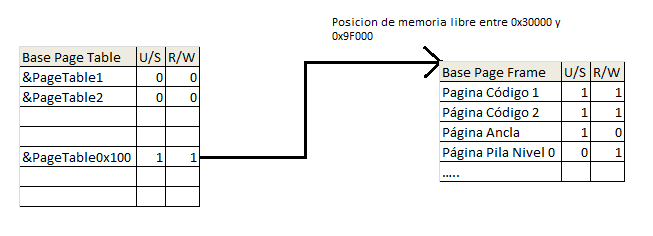
\includegraphics[scale=0.6]{imagenes/paginacionTareas.png}

Cabe destacar que para poder cumplir con los ejercicios siguientes, una tarea IDLE va a tener que ser mapeada al comienzo de la paginaci\'on
de lo contrario, no tener una tarea mapeada me imposibilita arrancar el sistema de scheduling que ser\'a introducido mas adelante.\footnote{Ver
secci\'on Ejercicio 7, Scheduling.}

\newpage
\subsection{Ejercicio 5 IDT / Clocks, Teclados y Syscalls}

La siguiente secci\'on est\'a dedicada a los \emph{Handlers} o manejadores de las interrupciones. Estos son los c\'odigos que se ejecutan
cuando alguna porci\'on del systema produce un error o llama a una interrupci\'on mejor conocida como syscall o servicios del sistema.\\
Nuestro Kernel cuenta con 3 interrupciones que poseen handlers. Estas fueron mencionadas en el punto 3. Procederemos a explicar cada una de
ellas:
\begin{itemize}
 \item Clock: El clock es una interrupci\'on que se ejecuta cada ciertos ticks de reloj. La misma se encarga de buscar el siguiente selector
de segmento según es especificado en la secci\'on 7. y realizar el salto a dicho selector que puede corresponder a una tarea, una bandera o 
la tarea IDLE.
 \item Teclado: La interrupci\'on de teclado cumple la funci\'on de cambiar el estado del juego.
 \item Servicios o Syscalls: Esta interrupci\'on brinda al systema una serie de servicios o funciones a las tareas:
  \begin{itemize}
   \item Minar: Estas minas destruyen a los tanques que se quieran mover a la posicion donde esta la mina.\\
   Las minas duran una sola vez, es decir, si un tanque es destruido por una mina, ́esta desaparece
(tambien es destruida). Las minas tambien pueden ser destruidas si un misil cae sobre la misma.\\
El unico parmetro de este servicio es la posicion donde colocar la mina. Un tanque puede colocar una mina 
en alguna de las 4 posibles direcciones a su alrededor de la posicion actual donde se encuentra.\\
Una vez llamado este servicio el scheduler desalojara al tanque y ejecutar a la proxima 
tarea mientras se encarga de colocar la mina anti-tanque en su lugar. \\
   \item Lanzar Misil: Los tanques tvenen ca ̃
nones que les permiten disparar balas a sus enemigos, ahora,
como los disparos seran dirigidos a posiciones precisas del mapa, los llamaremos misiles. \\
Dicho esto, este servicio permitir ́a lanzar misiles a posiciones de el mapa direccionadas
de forma relativa a la posicion del tanque. Los valores posibles para x e y no pueden
superar en modulo el tamaño maximo de el mapa, es decir 50.\\
El buffer donde se almacena el misil debe ser un rango dentro del area mapeada por la
tarea, ademas el tamaño del mismo no debe superar los 4096 bytes.\\
El servicio se debe encargar de copiar el buffer del misil dentro al principio de la pagina
fısica idenfiticada por las coordenadas x e y dentro de el mapa. Una vez lanzado el misil,
el scheduler dara paso a la proxima tarea.\\
   \item Mover: El codigo de cada tanque esta mapeado incialmente en dos paginas de memoria a 
   partir de la direccion correspondiente a los 128mb de memoria virtual. A partir de esta
direccion, luego de las dos paginas mapeadas inicialmente, se ir ́an mapeando las 
paginas de memoria f ́ısica que el tanque recorra. Si a la hora de mapear una nueva pagina
fısica, esta esta ya esta mapeada dentro del espacio del tanque, entonces no se mapea
nuevamente.
  \end{itemize}

\end{itemize}

Cabe destacar que las funciones implementadas en C para las syscalls, minar, misil y mover, se encuentran allí dado que manejan p\'aginas
de memoria haciendo que ubicarlas en mmu.c sea lo m\'as conveniente para aprovechar todas las funciones y estructuras utilizadas. 

\newpage
\subsection{Ejercicio 6. TSS}

Para que el procesador pueda despachar, ejecutar o suspender m\'ultiples tareas, es necesario salvar el estado de las mismas. La 
arquitectura provee mecanismos para esto. El segmento de estado (TSS, Task State Segment), es el que se encarga de almacenar la 
informaci\'on del estado de una tarea.\\

Una tarea est\'a identificada por el selector de segmento de su TSS. Y a su vez la TSS es un segmento, por lo tanto debe estar descripto 
en la GDT junto con los descriptores de segmento de c\'odigo y datos.\footnote{Ver secci\'on 1 para mas informaci\'on sobre esto.}\\

Tenemos 8 tareas y definimos un total de 2 TSS, y otro lo 
dejamos en blanco para la tarea inicial donde se hace el primer salto.\\

Al contar con dos TSS y 8 tareas realizamos cambios de contextos guardando los datos de las tareas con una estructura auxiliar, permiti\'endonos as\'i volver m\'as tarde a esa tarea y no perder la informaci\'on de la 
misma. El cambio de una tss a otra lo realizamos en nuestra estructura de scheduler ejecutando JMP FAR.\\
Por esto mismo es necesario''incializar'' una TSS para que cuando entremos por primera vez la informaci\'on
sea v\'alida. Al momento de inicializar estos segmentos, cada tarea tendran TSS virtualmente id\'enticas, con la excepci\'on del
 eip y pequeños cambios con respecto a las posiciones de las pilas.\\

Como selectores de segmentos de GDT usamos los que definimos para las tareas (es decir, los de nivel 3), y seteamos el RPL en 0x03 para 
evitar un GPE.\\

Una de las grandes ventajas de estar trabajando con direcciones virtuales es que no tenemos que saber la direcci\'on f\'isica exacta de
cada tarea para inicializarlas. Sabemos que todas las tareas comparten ciertas direcciones virtuales, asi que seteamos el directorio de 
p\'agina (CR3) correspondiente a esa tarea y podemos usar direcciones virtuales id\'enticas para todas las tareas. 
\\

\newpage
\subsection{Ejercicio 7. Scheduller}

El Scheduler es la estructura m\'as grande y quiz\'as m\'as compleja de nuestro trabajo. Su funcion es simple, coordinar en 
que orden ocurren los eventos en nuestro Kernel y determinar ciertas acciones como si una tarea es desalojada por una operacion ilegal o mina, o un cambio simple de tareas por tick de reloj.\\
Conceptualmente nos imaginamos al Scheduler teniendo:
\begin{enumerate}
 \item Un timer llamado quantum que dictamina cuantos ciclos le queda a la corrida de tareas hasta que vuelva a empezar.
 \item Un estado pause, que en caso de estar activo hara que corra solo la tarea Idle.
 \item Un array donde guardamos el contexto de todas las tareas incluyendo la Idle.
\end{enumerate}

Corrida tarea:\\
\begin{center}
%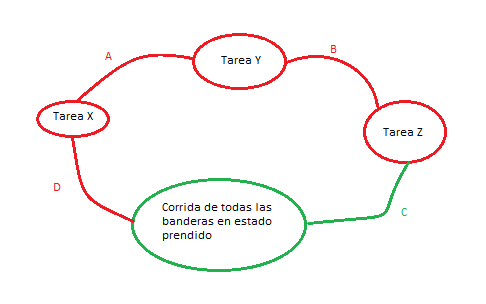
\includegraphics[scale=0.7]{imagenes/cicloBasicoTareas.png} 
\end{center}

\begin{center}
%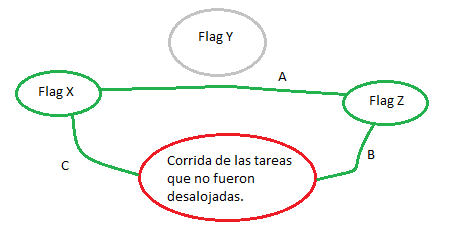
\includegraphics[scale=0.7]{imagenes/corridaFlags.png} 
\end{center}


La interrupci\'on de clock se encarga de realizar todos los saltos y cambios de tareas, exceptuando el salto a idle (que puede ser hecho 
en cualquier momento). El scheduler es la estructura que le informa hacia donde ir siguiendo. De esta forma, mantenemos el c\'odigo facilmente 
segmentado.\\

Una excepci\'on interesante es el caso en el que no querramos saltar a ningun lado sino seguir en la tarea actual. Por ejemplo, si me 
queda una sola tarea y estoy en la corrida de tareas a\'un con quantum me gustar\'ia pertenecer en esa tarea. Para esto el scheduler 
devuelve el selector de segmento 0, el cual es reconocido por el clock como una instrucci\'on para volver a la tarea anterior (iret) 
y no realizar ningun salto. (tratar de saltar a una tarea en uso daria error).


\newpage
\subsection{Screen}

La estructura screen tambi\'en es una parte integral del trabajo porque no solo se ocupa de mostrarle
la informaci\'on al usuario, en ella tambi\'en se guardan ciertos datos y se interpreta cierta informaci\'on.
Por esto mismo nos pareci\'o importante agregarle una secci\'on.\\
\\
Nuestra pantalla est\'a separada en 3 gr\'aficos distintos, el mapa, 
la tabla de contexto de tareas (que se encuentra en la parte derecha), la tabla de errores (que se encuentra en la parte inferior derecha) . Todas tienen su propias funciones, y la ventaja que tienen es que pueden ser chequeadas cuantas veces uno quiera presionando la respectiva tecla(Ver interrupcion Teclado).\\
\\
La tabla de contexto de tareas es una estructura que imprime el estado de una tarea, es decir los registros. En caso de que la tarea muera,
esto muestra el ultimo contexto activo antes de morir.\\


\newpage
\subsection{Game}
Para manejar toda la lógica del juego, los cambios en la pantalla y los mapeos correspondientes tenemos una estructura
llamada Game. Básicamente se encarga de las 3 posibles acciones de una tarea: minar, mover y lanzar misiles.
Tiene guardado internamente una matriz tablero, donde almacenamos el estado del juego actual. 
Ni bien comienza el juego, procedemos a inicializarlo: ponemos todos los valores de la matriz tablero en 0
y distruibuimos las tareas a lo largo y ancho del mapa. Para indicar que el tanque está en cierta posición,
en la matriz tablero ubicamos el número del tanque en la posición correspondiente.

\begin{enumerate}
 \item \textbf{Minar:} Recibimos la posición relativa al tanque que quiere minar y calculamos la posición que le corresponde
 al tablero y con esa, colocamos el valor -1 en el tablero (arbitrario, indica que es una mina) y la dibujamos en pantalla.
 \item \textbf{Misil:} Recibimos la posición relativa a donde lanzar el misil, y además recibimos la dirección desde dónde se copiará el misil (buffer)
 y su tamaño.
 Esta acción es similar a lo que llamamos virus, ya que en caso de caer dicho misil en una parte del código de otro tanque se lo pisará y cambiará,
 generando un posible error en ese tanque cuando vaya a ejecutarse.
 \item \textbf{Mover:} Para realizar esta función del juego utilizamos un struct tanque, el cual tiene su posición columna y fila.
 Lo que hacemos es incrementar o decrementa el valor fila y/o columna según corresponda la dirección pasada como parámetro.
 A su vez dentro de este struct tenemos la ultima dirección virtual mapeada, y se la aumentamos siempre y cuando se mueva a una posicion donde no estaba.
 En caso de haber una superposición con otro tanque no ocurrirá nada (solo se mostrara en pantalla con una x). En cambio si en esa posición 
 el tablero$_{[fila],[columna]}$ es igual a -1, el tanque explotará y dejara de andar, ya que como dijimos anteriormente el -1 indica 
 que hay una mina en esa posición..
\end{enumerate}

\newpage
%%%%%%%%%%%%%%%%%%%%%%%%%%%%%%%%%%%%%%%%%%%%%%%%%%%%%%%%%%%%%%%%%%%%%%%%%%%%%%%
%% Conclusión                                                                %%
%%%%%%%%%%%%%%%%%%%%%%%%%%%%%%%%%%%%%%%%%%%%%%%%%%%%%%%%%%%%%%%%%%%%%%%%%%%%%%%



\end{document}